\newpage
\section{Testowanie}
Testy automatyczne są bardzo ważną częścią każdej aplikacji. Pozwalają one w łatwiejszy sposób wprowadzać zmiany do naszej aplikacji mając większą pewność, że nasze zmiany nie wprowadziły niepożądanych błędów do naszego kodu. Dodatkowo podczas procesu pisania kodu naszej aplikacji, dzięki takim testom jesteśmy w stanie w łatwy sposób sprawdzić poprawność naszych rozwiązań w wielu różnych sytuacjach. 

W mojej aplikacji użyłem trzech różnych sposobów na przetestowanie mojej aplikacji:
\begin{enumerate}
  \item Testowania jednostkowego
  \item Testowania integracyjnego
  \item Wizualnej regresji
\end{enumerate}

\subsection{Testowanie jednostkowe aplikacji klienckiej}
Testowanie jednostkowe pozwala nam w prosty sposób przetestować poszczególne komponenty naszej aplikacji w izolacji. Komponenty w bibliotece React to zwykłe funkcje, więc można by pomyśleć, że możemy je testować jak funkcje, jednak jest kilka rzeczy, o których musimy pamiętać. 

\subsubsection{Testowanie komponentów}
Jednym z powodów dla którego trudno jest testować komponenty jak zwykłe funkcje jest to, że komponenty mogą posiadać stan. Jak widać w listingu \ref{lst:reactCounterCode} używając funkcji \emph{React.useState} dołączamy do funkcji stan, który może się różnić przy różnych wywołaniach danego komponentu. Z tego powodu kolejne wywołania tej samej funkcji mogą zwracać inny wynik. 

Kolejnym powodem, dla którego trudno by było przetestować komponent bazując tylko i wyłącznie na jego zwróconym wyniku jest to, że wartością zwracaną przez komponent jest zwykły obiekt, który reprezentuje część wirtualnego DOM'u. Natomiast my jako programiści interpretujemy tę część wirtualnego domu jako prawdziwe elementy przeglądarki, dlatego asercje, które sprawdzały by poprawność wirtualnego DOM'u mogłyby być nieczytelne i trudne w utrzymaniu.

Dodatkowo nasze komponenty mogą używać interfejsu przeglądarki, więc aby w całości przetestować komponent musimy być w stanie też sprawdzić jak komponenty wchodzą w interakcje z przeglądarką.

Aby móc poprawnie jednostkowo przetestować moje komponenty użyłem do tego dwóch bibliotek: \emph{react-testing-library} \cite{ref_rtl_doc} oraz \emph{jest} \cite{ref_jest_doc}.

\subsubsection{Jest} Jest jest biblioteką, która udostępnia programiście interfejs, dzięki któremu możemy testować każdy kod javascript, w tym w szczególności komponenty React. Aby zasymulować środowisko przeglądarki Jest używa sztucznego środowiska o nazwie \emph{jsdom}, dzięki któremu możemy testować nasz kod w środowisku, w którym nasz kod Javascript będzie wykonywany, czyli przeglądarce. Biblioteka Jest została stworzona przez Facebook'a i jest nadal rozwijana. 

Jest posiada dużo funkcji, które ułatwiają testowanie kodu Javasrcipt.
\begin{description}
  \item[Interfejs do tworzenia asercji] \hfill \\ Jest udostępnia prosty i zrozumiały interfejs dzięki któremu możemy tworzyć bardzo czytelne testy. Nazwy asercji są bardzo intuicyjne i czyta się je jak prawdziwe zdania w języku angielskim.
  \begin{addmargin}[6mm]{0mm}
  \begin{lstlisting}[
      numbers=left,
      firstnumber=1,
      caption={Przykład testu napisanego w bibliotece Jest},
      aboveskip=10pt
  ]
  test('funkcja powinna byc zawolana', () => {
    // zakladajac
    let funkcja = jest.fn();

    // kiedy
    funkcja(); 

    // wtedy
    expect(funkcja).toEqual(funkcja);
    expect(funkcja).toHaveBeenCalledTimes(1);
  })
  \end{lstlisting}
  \end{addmargin}

  \item[Równoległe uruchamianie testów] \hfill \\ Jest pozwala na uruchamianie testów jednocześnie na wielu wątkach, przez co testy wykonują się nawet kilka razy szybciej, niż gdyby odpalało się je pojedynczo.
  \item[Migawki] \hfill \\ Jest udostępnia nam interfejs, dzięki któremu możemy tworzyć tzw. migawki (ang. snapshots). Migawki są techniką pozwalającą testować zmiany, które mogły nastąpić pomiędzy następnymi uruchomieniami testów.
  \begin{addmargin}[6mm]{0mm}
  \begin{lstlisting}[
      numbers=left,
      firstnumber=1,
      caption={Przykład testu migawkowego},
      aboveskip=10pt
  ]
  function funkcjaDoMigawki() {
    return '<div>Witaj swiecie!</div>';
  }

  test('funkcja powinna zwracac poprawny wynik', () => {
    expect(funkcjaDoMigawki).toMatchSnapshot();
  })
  \end{lstlisting}
  \end{addmargin}
  W powyższym teście widzimy że funkcja \emph{funkcjaDoMigawki} zwraca nam taga \emph{div} z tekstem w środku. W naszym teście moglibyśmy sprawdzić zawartość zwróconej wartości przez funkcję, lecz wymagałoby to od nas ręcznego wpisania wartości w asercji. W naszym przypadku jest to jedna linijka, ale w przypadku komponentów React, które mogą zwracać nawet kilkadziesiąt linijek wpisywanie ręczne zwracanej wartości mogłoby się okazać dosyć trudnym zadaniem.

  Migawki rozwiązują ten problem. \emph{toMatchSnapshot} podczas pierwszego uruchomienia zapamiętuje wartość zwróconą przez funkcję, a przy następnych uruchomieniach testu sprawdza, czy wynik zgadza się z wynikiem z poprzedniego uruchomienia. Jeżeli te dwie wartości nie będą się zgadzać, Jest zwróci programiście, że test nie przeszedł. W takiej sytuacji programista może zaakceptować nowy wygląd migawki, lub poprawić błąd jeżeli zmiana była niezamierzona. Takie testy są właśnie stworzone po to, aby nie wprowadzać niepożądanych zmian do naszego kodu aplikacji.

\subsubsection{React-testing-library} React-testing-library natomiast rozwiązuje problem czytelności i łatwości testowania naszych komponentów. Dzięki tej bibliotece jesteśmy w stanie testować zachowanie naszych komponentów używając do tego bardzo prostego interfejsu, który pozwala nam na wykonywanie takich operacji jak:
\begin{itemize}
  \item łatwe tworzenie komponentów w wirtualnym środowisku
  \item wykonywanie akcji użytkownika np. klikanie, najeżdżanie myszką itp.
  \item łatwe wyszukiwanie elementów i sprawdzanie ich stanu lub atrybutów
\end{itemize}


\end{description}
  \begin{addmargin}[6mm]{0mm}
  \begin{lstlisting}[
      numbers=left,
      firstnumber=1,
      caption={Przykład testu jednostkowego przy użyciu React-testing-library},
      aboveskip=10pt
  ]
    test('gdy nazwa wydatku jest za dluga powinien pojawic sie blad', () => {
    // given
    const { getByLabelText, queryByText } = render(<FormularzWydatku />);

    // when
    const poleZNazwa = getByLabelText('Nazwa wydatku');

    await userEvent.type(poleZNazwa, 'x'.repeat(51));

    // then
    const blad = queryByText(
      "Pole nie moze miec wiecej niz 50 znakow."
    );

    expect(blad).toBeInTheDocument();
  });
  \end{lstlisting}
  \end{addmargin}
  W powyższym teście możemy zauważyć, że symulujemy wpisywanie do pola \emph{Nazwa wydatku} 51 znaków, a następnie sprawdzamy, czy w naszym komponencie wyświetlił się poprawny błąd. Dzięki takim testom komponentów, możemy w łatwy sposób przetestować zachowanie komponentów w wielu różnych scenariuszach.

Testowanie jednostkowe ma natomiast kilka limitacji:
\begin{itemize}
  \item nie pozwalają sprawdzać integracji aplikacji z serwisami zewnętrznymi np. komunikacji z serwerem
  \item jako, że Jsdom tylko symuluje środowisko przeglądarki, w aplikacji mogą pojawiać się błędy, które pojawiają się w prawdziwej przeglądarce. Takich błędów testy jednostkowe nie są w stanie wyłapać
\end{itemize}

\subsection{Testowanie integracyjne aplikacji klienckiej}
Testowanie integracyjne pozwala nam rozwiązać te wyzwania, które wystąpiły przy testowaniu jednostkowym. 

Do testów integracyjnych użyłem biblioteki o nazwie \emph{Cypress.io} \cite{ref_cypress_doc}. Biblioteka ta pozwala nam pisać testy, które potem są wykonywane w prawdziwej instancji przeglądarki. Cypress udostępnia nam interfejs, dzięki któremu możemy wykonywać akcje użytkownika (np. wpisywanie tekstu, klikanie itp.). Pozwala nam ona także sprawdzać poprawne działanie zewnętrznych serwisów jak i komunikację z nimi. 

  \begin{addmargin}[6mm]{0mm}
  \begin{lstlisting}[
      numbers=left,
      firstnumber=1,
      caption={Przykład testu integracyjnego z użyciem bilbioteki Cypress},
      aboveskip=10pt
  ]
  it('wydatek powinien sie usunac', () => {
    // register
    cy.visit('/login');
    logIn(1);

    // create new expense
    cy.contains('Przykladowy opis zmieniony').click();
    cy.contains('Usun').click();
    cy.contains('OK').click();

    cy.contains('Przykladowy wydatek zmieniony').should('not.exist');
    cy.contains('Przykladowy opis zmieniony').should('not.exist');
  });
  \end{lstlisting}
  \end{addmargin}
  W powyższym przykładzie mamy przedstawiony przykładowy test integracyjny naszej aplikacji. Przy użyciu intefejsu Cypress możemy sterować przeglądarką i tworzyć testy które symulują prawdziwego użytkownika w prawdziwej instancji przeglądarki.

Cypress udostępnia nam też podgląd testów \emph{na żywo}. Dzięki temu, gdy test nie przejdzie, jesteśmy w łatwy sposób stwierdzić gdzie jest błąd i jak go naprawić.

\begin{figure}
    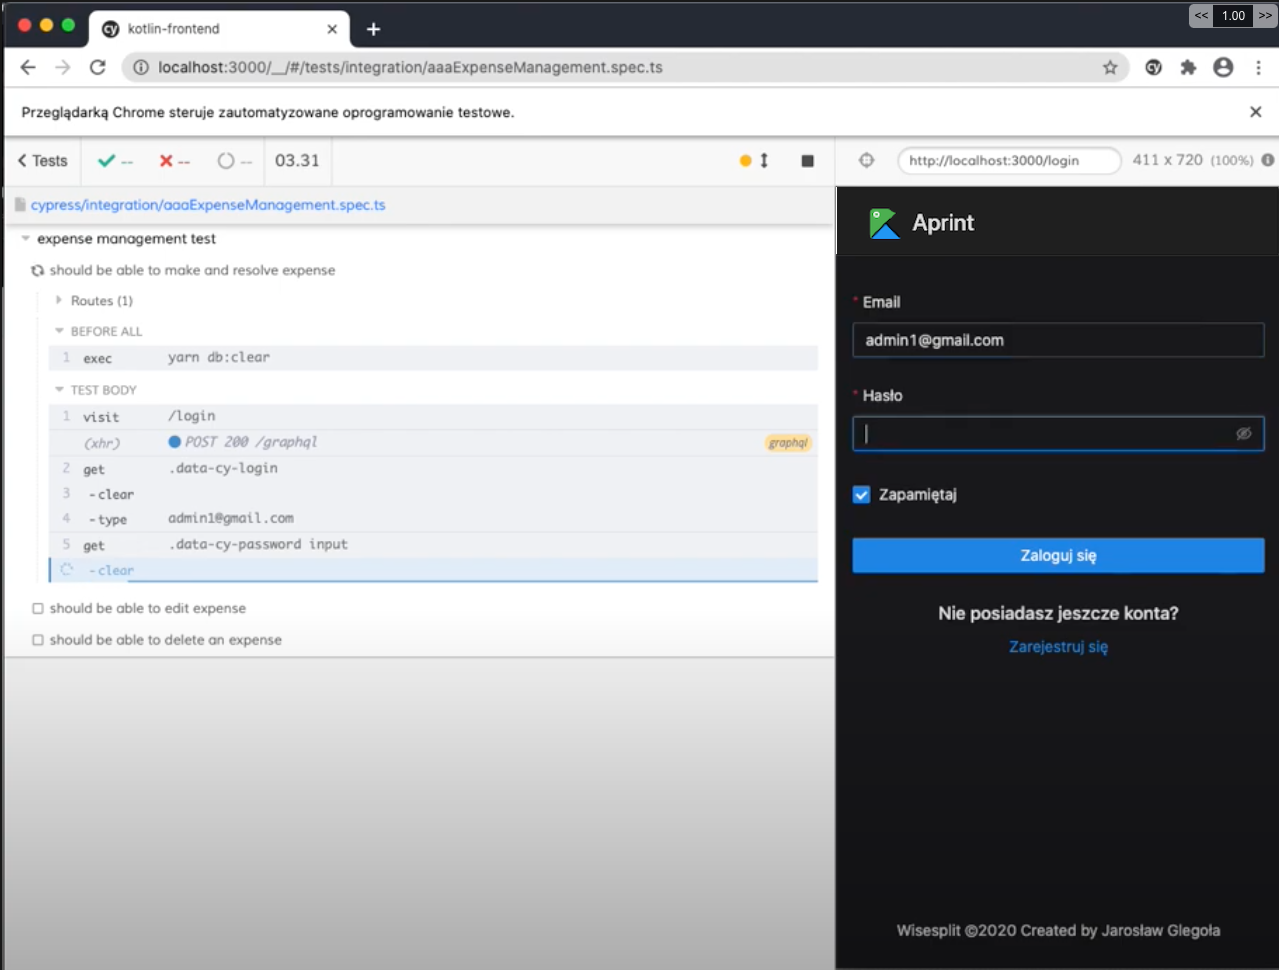
\includegraphics[width=\textwidth]{cypress-imape.png}
    \caption{Rysunek przedstawia panel Cypress.io. Możemy w nim zauważyć po lewej stronie komendy, które są po kolei wykonywane, a po prawej stronie wynik wykonania tych komend w prawdziwej instancji przeglądarki.} \label{fig-cypress}
\end{figure}

\subsection{Testy wizualnej regresji aplikacji klienckiej}
Testy wizualnej regresji zapewniają nam wizualną poprawność naszego interfejsu użytkownika. Dzięki nim mogłem programatycznie symulować sytuacje biznesowe, a następnie przy pomocy biblioteki Cypress.io robić zrzuty ekranu. Testy wizualnej regresji działają podobnie jak testy migawkowe, tylko zamiast zapamiętywania wartości zwóronej przez funkcję Cypress zapamiętuje zrzut ekranu przeglądarki. Gdy pierwszy zrzut ekranu aplikacji został zrobiony podczas pierwszego uruchomienia testu, każde następne uruchomienie tego samego testu będzie robiło kolejny zrzut, a następnie porównywało z poprzednim. W taki sposób możemy sprawdzać, czy po naszych zmianach w kodzie nie nastąpiła niepożądana zmiana w wyglądzie naszej aplikacji. Jeżeli takie dwa zrzuty się różnią, test wyświetli nam komunikat błędu a następnie wyświetli nam różniące się zrzuty ekranu i wyróżni wszystkie różniące się pixele obu zdjęć.

\begin{figure}
    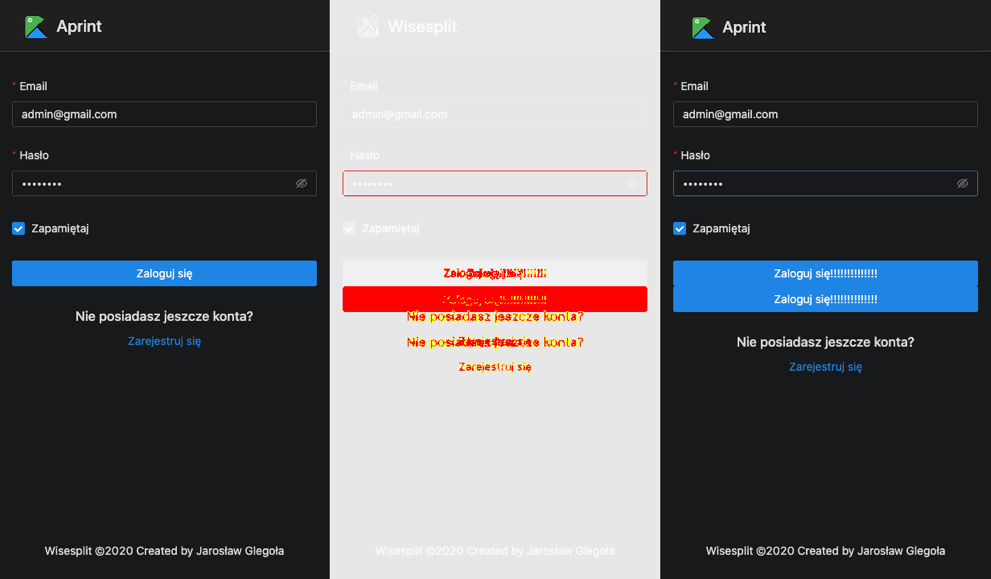
\includegraphics[width=\textwidth]{wisual-regression.png}
    \caption{Przykład testu wizualnej regresji, w którym możemy zobaczyć dokładnie, które pixele różniły się pomiędzy poszczególnymi uruchomieniami testu} \label{fig-cypress-vr}
\end{figure}


\subsection{Testy integracyjne aplikacji serwerowej}
Aplikację serwerową testowałem głównie integracyjnie. Do pisania testów wybrałem język Groovy i bibliotekę Spock w środowisku JUnit. Testy integracyjne serwera nie róznią się w dużej mierze od testów integracyjnych aplikacji klienckiej. Jedyną różnicą jest to, że nie posiadamy wizualnej części. Testy integracyjne testują wszystkie elementy aplikacji serwerowej: zapytania klienckie, logikę biznesową oraz integrację z bazą danych.
